\chapter{An overview of the events}
\label{ch:events}

\begin{instructions}
About 5 pages. This is the chapter your supervisor reads: spike- and event-level statistics, families, scale and
species. Sources:
\begin{itemize}
  \item \src{docs/rq_roundA_2/findings/catalogue-stats-2026-10-26.md} (recomputed 26 Oct, read-only);
  \item the spiking-families pass of 19 Aug (the MJu26a CH14 excerpt, 4\,h);
  \item \src{docs/rq_roundA_2/findings/library-fragments-and-duplicates.md} and the 26 Oct grouping survey;
  \item the drop-motif study: \src{Plots/drop_motifs10/CLAIMS.md} and \src{Plots/drop_motifs12b/FIGURES.md}, whose
        captions are ready to paste;
  \item \src{docs/rq_roundB/notes/drop-motif-sequences.md}.
\end{itemize}
Present single-recording results as case studies, not as facts about fungi.
\end{instructions}

\section{Aims}

The research questions test the instrument. This chapter uses it to describe what it found: the size, duration, polarity and timing of the events a human accepted, how they group into families, and how far shape survives a change of scale and species. Its descriptions are the raw material for the morphology vocabulary (Appendix~\ref{app:vocab}) and for the spiking-family taxonomy the supervisor proposed.

\section{The catalogue of accepted events}
\label{sec:catalogue}

\begin{figure}[htbp]
\centering
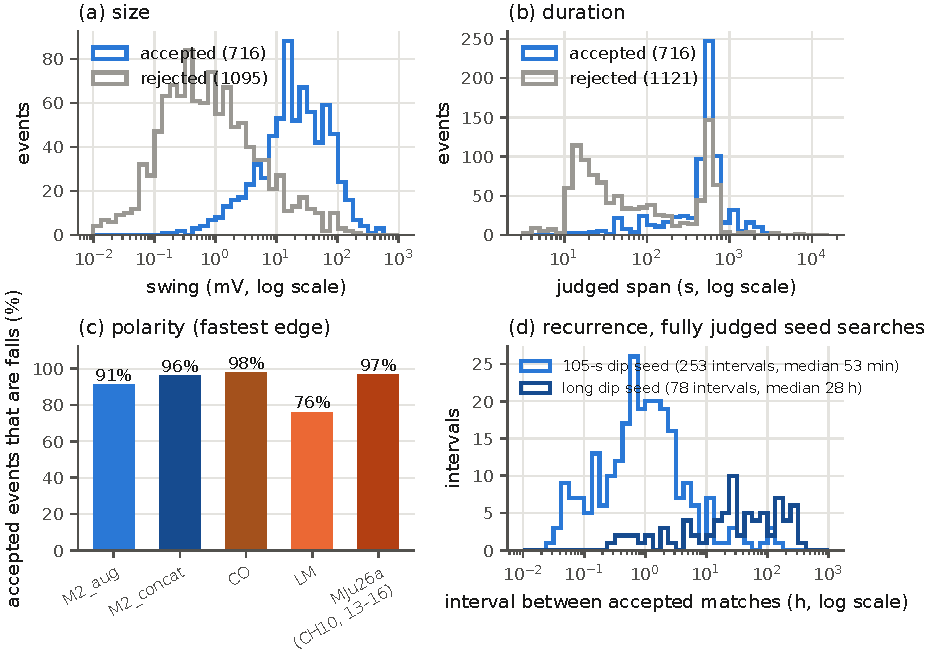
\includegraphics[width=\textwidth]{new/ch9_catalogue.pdf}
\caption{The judged events of the blind queues (25 and 28, five recordings). (a) Swing and (b) judged span length, accepted against rejected: accepted events are larger, and many spans are about 600\,s because detectors frame them that way. (c) The share of accepted events whose fastest edge is a fall, per recording. (d) Intervals between accepted matches on one channel, for the two seed searches judged in full.}
\label{fig:catalogue}
\end{figure}

\begin{figure}[htbp]
\centering
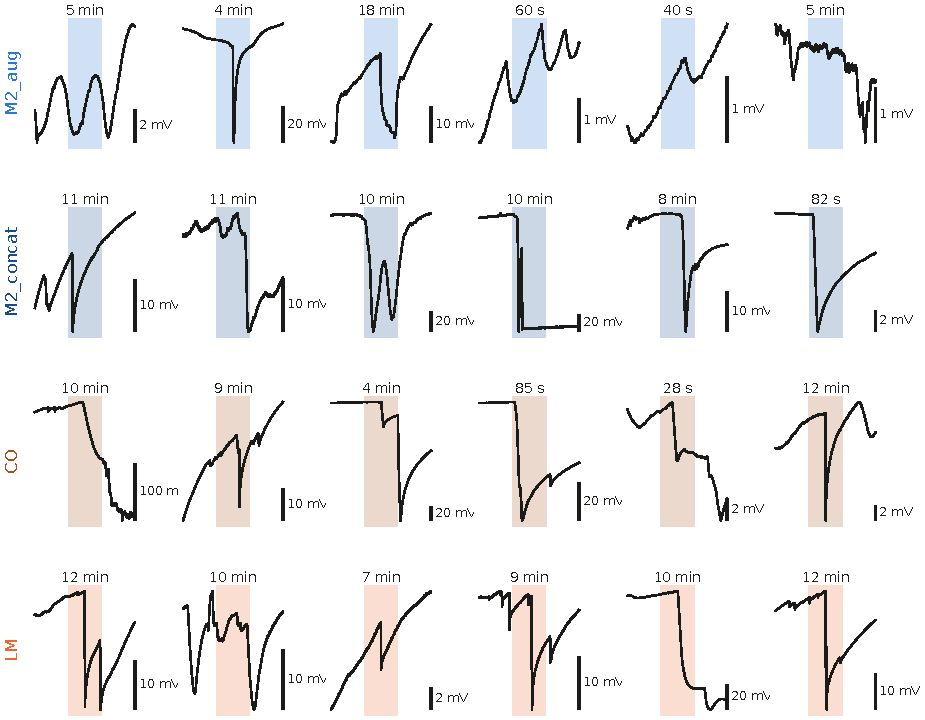
\includegraphics[width=\textwidth]{new/ch9_accepted_gallery.pdf}
\caption{What an accepted event looks like: six accepted events from each of four recordings, drawn at random, each with its own length of context either side. Each panel has its own scale; the bar gives millivolts and the title the event's length. Most are falls in potential, from seconds to tens of minutes long and from a few to a hundred millivolts deep.}
\label{fig:acceptedgallery}
\end{figure}

\begin{instructions}
The recomputed numbers. Use these, not the poster's:
\begin{itemize}
  \item \textbf{swing}: median 19.8\,mV, 14--30\,mV per recording; top 5\,\% above 122\,mV; smallest 0.17\,mV;
  \item \textbf{duration}: median 603\,s (5--95\,\%: 40--1,272\,s). Much of this is detector framing: 24\,\% of spans
        are about 600-s windows. Say so. The poster's ``several hours'' does not reproduce; the maximum is about 2\,h;
  \item \textbf{polarity}: 68\,\% of accepted events are falls in potential pooled, 57--80\,\% per recording, against
        about half of rejected candidates. The poster's ``73\,\% (56--86\,\%)'' does not reproduce. The tool's own
        fastest-edge rule (\texttt{event\_shape} auto) gives 91\,\% pooled, 76--98\,\% per recording. The earlier
        ``9\,\%'' here was a sign error in the statistics script, fixed on 3 Nov. State which rule you use;
  \item \textbf{size against judgement}: accepted events are much larger than rejected ones. This is partly circular,
        because size is one thing you judged by: it describes what ``an event'' meant in practice;
  \item \textbf{recurrence}: intervals mean something only for the fully judged seed searches. The 105-s dip recurs
        with a median of 53 minutes, and in bursts.
\end{itemize}
\end{instructions}

\section{One recording in detail: spiking families}
\label{sec:spikingfamilies}

\begin{instructions}
The 19 Aug spiking-families pass on the MJu26a CH14 excerpt (4\,h, 1\,Hz). It was made for the
supervisor's Izhikevich-style taxonomy. Findings, as a case study:
\begin{itemize}
  \item the 1-minute matrix-profile scale suits single spikes; at 3 and 10 minutes the window is mostly baseline;
  \item two amplitude regimes, about 7--14\,mV peak to peak and a separate sub-mV mode at about 0.4--0.6\,mV;
  \item some families are amplitude-stereotyped (s.d.\ of peak to peak about 0.15\,mV), others are not (1.6--3.1\,mV);
  \item the median inter-occurrence interval is 900--1,400\,s.
\end{itemize}
Add the later \texttt{motif\_lengths} result: on the MJu26a CH14 excerpt every judged length from 30\,s to 16\,min
repeats beyond AAFT noise, strongest at 30\,s. So the pan picture, not a single window, is where a scale is read
(\src{docs/prompts/blocks/reports/W3-evaluation.md}). Use the overlay figure from the motif report tool if you want a
picture of a family.
\end{instructions}

\begin{figure}[htbp]
\centering
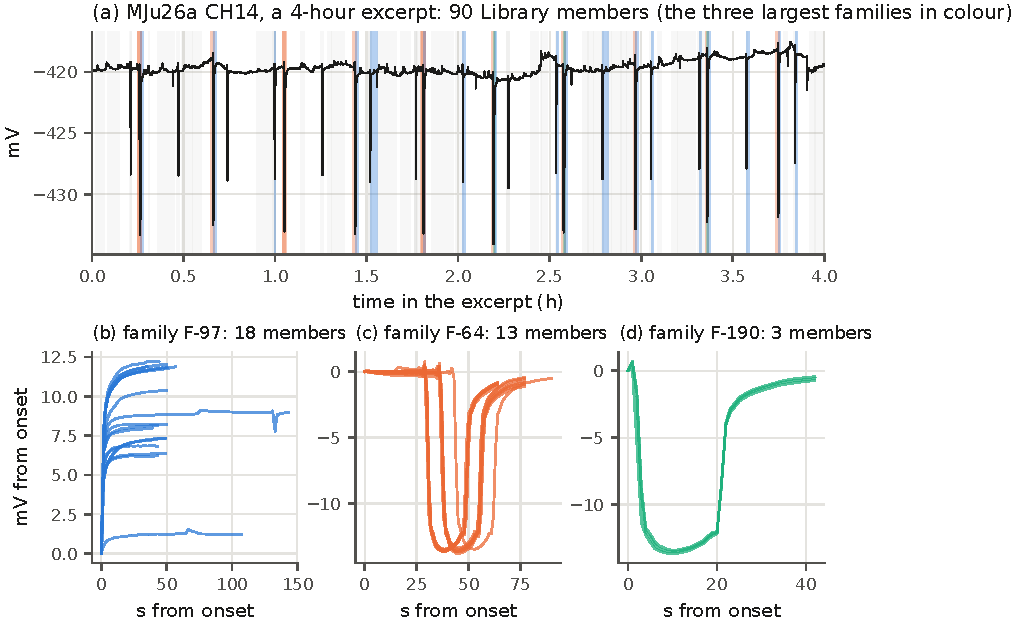
\includegraphics[width=\textwidth]{new/ch9_rec385.pdf}
\caption{One recording in detail. (a) The 4-hour excerpt of MJu26a CH14 with its 90 Library members shaded, the three largest shape families in colour. (b--d) The members of each of those families drawn from their onsets: the same shape recurs throughout the four hours.}
\label{fig:rec385}
\end{figure}

\section{Shape families in the Library}
\label{sec:families}

\begin{figure}[htbp]
\centering
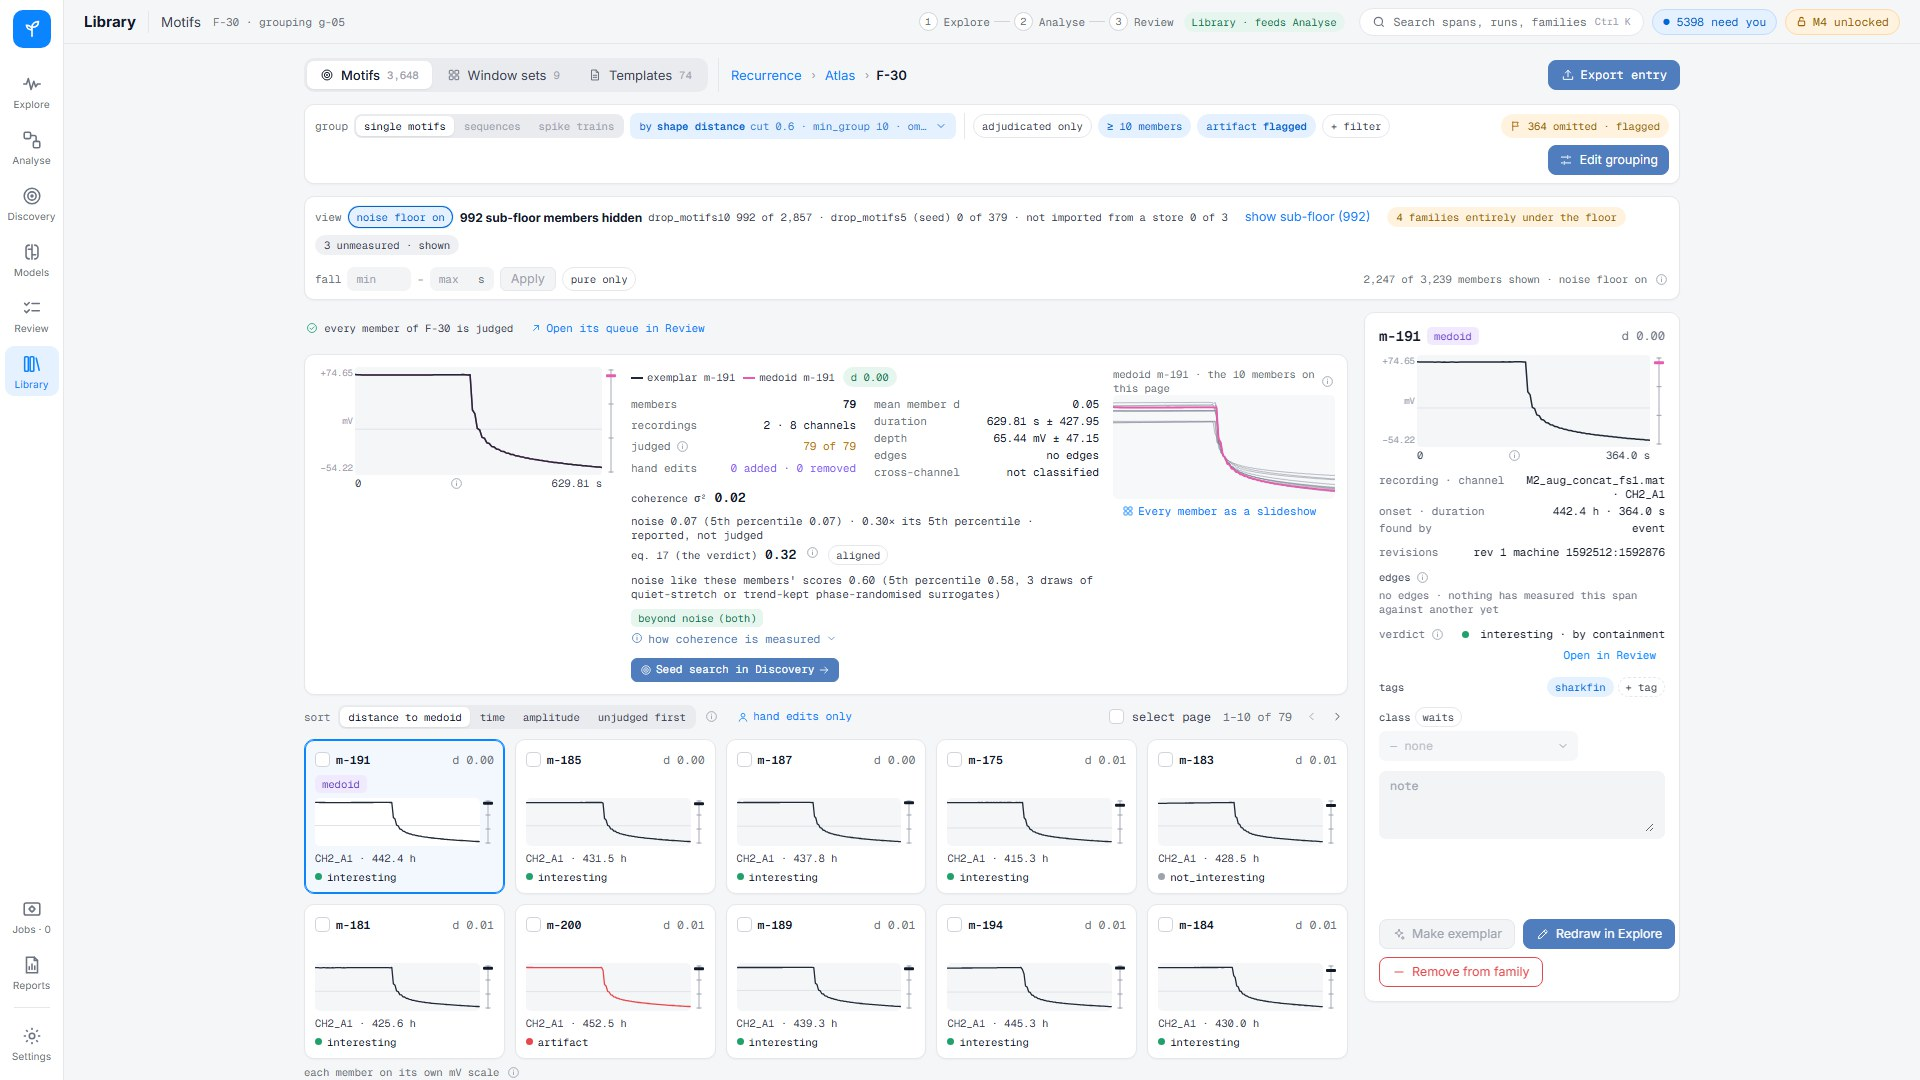
\includegraphics[width=\textwidth]{screens/library_family_f30.jpg}
\caption{One Library family (F-30, grouping g-05): 79 members around their medoid, all judged.}
\label{fig:familyf30}
\end{figure}

\begin{instructions}
Grouping g-05 (Ward on the resampled, z-normalised, scale-invariant distance; cut 0.60; minimum 10; omit distance
0.5):
\begin{itemize}
  \item 149 families from 3,239 assigned members (364 omitted); family size median 18 (10--79);
  \item 67\,\% of members are overlapping 2-second pieces of one 20-minute reishi recording (F2A), dominating 115
        families;
  \item human review: 247 Library verdicts (210 interesting, 35 not, 1 unsure, 1 artifact). The 210 accepted members
        are 144 events under the events rule below (152 by the earlier audit's pairwise $\ge$50\,\% overlap rule),
        in 11 families;
  \item the tree is fragile: a 1\,\% jitter of the waveforms changes membership to an ARI of 0.78--0.80, and 2\,\% to
        0.68--0.74. The 21 Sep re-derivation (about 3\,\%) gave ARI 0.57 against the stored g-05.
\end{itemize}
Report this honestly, as a finding about the method: a Ward cut is an imposed grouping, not a discovered partition.

Two event groupings were built for the thesis. The first is \textbf{g-10} (26 Oct), ``thesis · events · de-duplicated'':
\begin{itemize}
  \item Partial motifs are first joined into events (\src{scripts/thesis/library_events.py}): twins collapsed;
        containers kept with their parts; units joined at $\ge$50\,\% overlap or gaps $\le$3\,s, never through a
        container. 3,603 members become 1,116 events. Outside F2A, 1,178 become 590, and 35\,\% of those events span
        two or more g-05 families.
  \item One representative per event outside F2A and the Review regions is grouped with Ward as for g-05: 590 items
        give 25 families (410 assigned, 180 omitted). 8 families hold both recordings.
  \item Stability: wobble ARI 0.96 at 1\,\% jitter and 0.93 at 2\,\%, against 0.73--0.78 and 0.68--0.72 for the same
        test on all members. Part of the gain may simply be fewer items. Cophenetic correlation 0.66.
  \item Your 210 accepted members are 144 events. 80 of the 113 outside F2A are assigned, in 13 families.
  \item g-10 holds only M2\_aug and the MJu26a CH14 excerpt (4\,h, lion's mane). Its 8 two-recording families
        are therefore oyster--lion's mane overlaps.
\end{itemize}
The second is \textbf{g-11} (27 Oct), ``thesis · events · all active datasets''. Before it was built, the accepted events
of blind queues 25 and 28 were filed in the Library without a second verdict (\texttt{promote\_to\_library} in
\src{Working/review/promotion.py}): 600 promoted, 30 skipped as duplicates, and 86 refused because they sit on the
inactive 2\,Hz copy of MJu26a (CH10, 13--16). No verdict rows were written.
\begin{itemize}
  \item Every active recording except M4: 1,689 members join into 1,097 events (M2\_aug 830, LM 100, CO 93,
        M2\_concat 74), grouped as for g-10.
  \item 42 families (817 assigned, 280 omitted). 39 hold two or more recordings, and 14 hold all four.
  \item Stability: wobble ARI 0.93 (0.90--0.95) at 1\,\% jitter and 0.88 (0.86--0.91) at 2\,\%; cophenetic correlation
        0.65.
  \item 678 events hold an accepted member; 519 of them are assigned, in 41 families.
  \item Limitations:
        \begin{itemize}
          \item the MJu26a CH14 excerpt is inactive and MJu26a's own sweep is not judged, so g-11 holds nothing of
                MJu26a;
          \item species were unset for CO, LM and M2\_concat when g-11 was built. By Table~\ref{tab:corpus}, a family
                is cross-species only if it holds LM (lion's mane) and an oyster recording; CO is an oyster strain;
          \item on CO, LM and M2\_concat every member is an accepted detector event, so recurrence there is of what
                the detectors found and you kept.
        \end{itemize}
\end{itemize}
g-11 is the final grouping for this chapter and Chapter~\ref{ch:roundb} (5 Nov). Sources:
\src{docs/thesis/data/library_events/} (g-10) and \src{docs/thesis/data/library_events_all_active/} (g-11).
\end{instructions}

\section{Events no one has judged}
\label{sec:pool}

\begin{instructions}
New (5 Nov), first in the cut order. How many events would the Library hold if every candidate that five or more
detector families agree on were counted, and do they look like the accepted ones? Facts so far
(\src{docs/thesis/data/ledger_checks.json}): 1,720,104 candidates have $\ge$5 agreeing families across the five swept
tables, or 1,390,695 without the five-channel MJu26a copy; at 5--6 families only 7--22\,\% were real when judged, and
at 9 or more 40--63\,\%. Candidates nest, so the wave-1 run collapses them first (keep a candidate unless half its span
is covered by a higher-agreement one) and then measures a stratified sample of 2,000 per recording with the same
function as the catalogue, scored by R4. These are machine proposals: none of them enters the Library.

\textbf{Results (wave 1, 5 Nov; \src{DATA/derived/thesis_bundle/wave1}, pool step):}
\begin{itemize}
  \item \textbf{How many.} Merging nested candidates shrinks the pool about 27-fold: 5+ agreeing families, 1,720,104
        candidates become 64,114 events (M2\_aug 24,904; M2\_concat 21,253; MJu26a (CH10, 13--16) 9,890; CO 4,184;
        LM 3,883); 9+ agreeing, 230,817 become 10,620. The Library holds 1,097. MJu26a's 16-channel 2\,Hz sweep has no
        table yet, so its five-channel copy stands in.
  \item \textbf{What they look like.} The pool is smaller and shorter than what you accepted, and grows towards it with
        agreement: median swing 0.2--1.0\,mV at 5--6 families, 1.1--3.3\,mV at 7--8, and 14--17\,mV at 9+ on M2\_aug,
        CO and LM (accepted: 19.8\,mV). Many merged events are 10--60\,s fragments, because merging keeps the shortest
        high-agreement span.
  \item \textbf{What R4 makes of them.} R4 calls 11--18\,\% of the 5--6 tier an event, 31--43\,\% at 7--8, and 24--66\,\%
        at 9+ (M2\_aug 53, M2\_concat 34, CO 66, LM 61, MJu26a 24\,\%), close to the share you judged real at 9+
        (Figure~\ref{fig:ladder}). A rough scale: if R4 is right, about 4,500 of the 10,620 top-tier events are real,
        four times the Library.
  \item \textbf{Seeds.} On M2\_aug, 27\,\% of the sampled pool events overlap a seed-search match; elsewhere almost none
        do, because the seed searches ran on M2\_aug.
\end{itemize}
\end{instructions}

\begin{figure}[htbp]
\centering
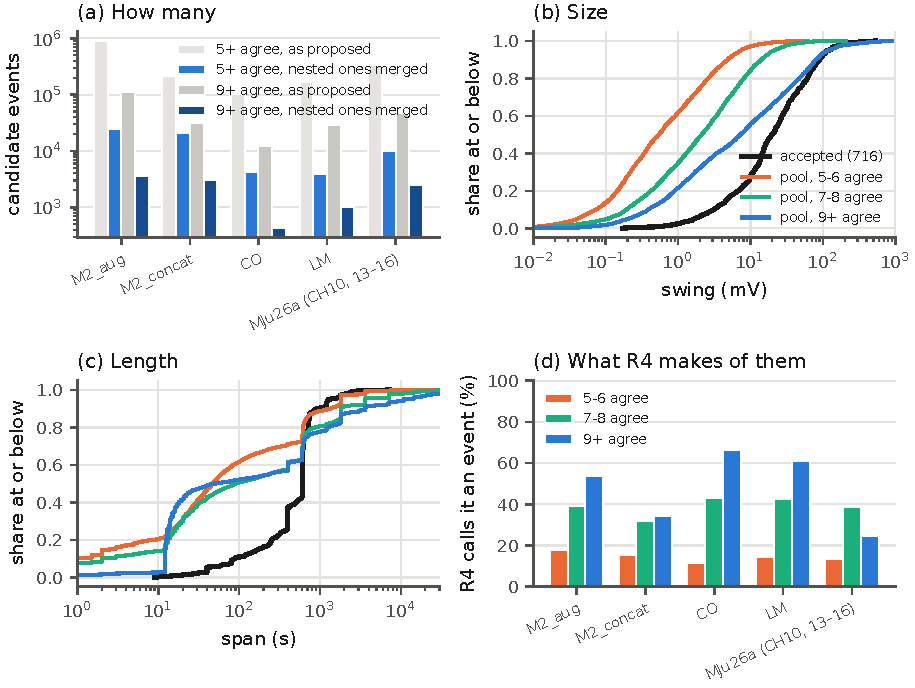
\includegraphics[width=\textwidth]{new/ch9_pool.pdf}
\caption{Events no one has judged. (a) Candidates on which five or more, and nine or more, detector families agree, as proposed and after merging nested ones (log scale). (b, c) The size and length of a stratified sample of 2,000 merged candidates per recording, by agreement, against the 716 accepted events (cumulative shares). (d) The share the frozen R4 classifier calls an event, by agreement.}
\label{fig:pool}
\end{figure}

\section{Discussion}

\begin{instructions}
Points to argue:
\begin{itemize}
  \item What generalises across recordings: drops dominate; the size and duration ranges.
  \item What is a case study: the MJu26a CH14 excerpt's amplitude regimes.
  \item What the vocabulary can and cannot rest on: a Ward cut is not a taxonomy, and normalised shape carries
        resolution, so shape names must be checked at matched rates.
  \item Which morphology tags have a measurable counterpart: sharkfin as dSAX \texttt{U+ S? D+}; drop as the drop
        detector; spike as the inverted drop detector.
\end{itemize}
\end{instructions}
